\chapter{The Likelihood and Maximum Likelihood}
\label{ch:likelihood}

\begin{chaptergoals}
\begin{itemize}[nosep]
\item The likelihood: the probability (or density) of the data you actually observed, read as a function of the parameter. One formula, two readings, and why the switch between them is the whole idea.
\item Why a density can stand in for a probability when the data are continuous.
\item The likelihoods of the standard families: Bernoulli, Poisson, Gaussian, exponential, uniform, and a mixture of Gaussians.
\item The maximum likelihood estimator, and how to find a maximum: concave functions, the first-order condition, and the second-derivative test in one and in several variables.
\item The maximum likelihood estimators of the standard families, computed for the kiss data, the siblings data, the subway data and the boarding data. The uniform family, where calculus fails and the answer is the largest observation.
\item When the estimator doesn't exist or isn't unique, and what to do when there is no formula: the EM algorithm for a mixture, run on the waiting times of Old Faithful.
\end{itemize}
\Cref{ch:distances} ended with a principle: minimizing an estimate of the KL divergence from the truth is the same as maximizing $\prod_i p_\theta(X_i)$. This chapter names that product and learns to maximize it.
\end{chaptergoals}

\section{From the KL divergence to the likelihood}
\label{sec:lik-from-kl}

\recall{\Cref{ch:distances}: for data $\Xton \iid \Pr_{\theta^*}$, $\KL(\Pr_{\theta^*}, \Pr_\theta) = \text{constant} - \E_{\theta^*}[\log p_\theta(X)]$; the Law of Large Numbers estimates the expectation by $\frac1n \sum_i \log p_\theta(X_i)$ (when $\log p_\theta(X)$ has finite variance); and the $\theta$ that minimizes the estimated divergence is the $\theta$ that maximizes $\prod_{i=1}^n p_\theta(X_i)$.}

That product is the subject of this chapter.
It is the probability, or the density, of the data you have, computed as if $\theta$ were the truth.
\Cref{ch:distances} reached it from a question about distances.
There is a second road to it, more direct and older.
Ask of each candidate $\theta$: if this were the truth, how probable would the data I actually saw be?
A candidate under which your data would be a fluke is a poor candidate.
A candidate under which your data are typical is a good one.
Ranking candidates by the probability they give your data, and picking the top one, is maximum likelihood.
The two roads arrive at the same estimator, and \cref{ch:mle-properties} uses the first one to prove that it works.

\section{The likelihood of a discrete model}
\label{sec:lik-discrete}

Start with a model whose observations take values in a countable set $E$: the kiss data in $\{0, 1\}$, the siblings counts in $\{1, 2, 3, \ldots\}$.
Each $\Pr_\theta$ has a PMF $p_\theta(x) = \Pr_\theta(X = x)$.

\begin{definition}[Likelihood, discrete model]
\label{def:likelihood-discrete}
Let $(E, (\Pr_\theta)_{\theta \in \Theta})$ be a statistical model for $\Xton$ i.i.d., with $E$ countable and $\Pr_\theta$ having PMF $p_\theta$.
The \textbf{likelihood} of the model is the function
\begin{align*}
L_n : E^n \times \Theta &\to \real \\
(x_1, \ldots, x_n; \theta) &\mapsto \Pr_\theta(X_1 = x_1, \ldots, X_n = x_n) = \prod_{i=1}^n p_\theta(x_i).
\end{align*}
The product form is independence: the joint PMF of independent observations is the product of the individual PMFs.
We write $L$ for $L_n$ when $n$ is clear, and $L(\theta)$ when the data are fixed.
\end{definition}

\begin{inwords}
\textbf{In words.} Take the data you observed and a candidate $\theta$, and compute the probability that the model with parameter $\theta$ would produce exactly those data. That number, for every candidate at once, is the likelihood. The data are held fixed; the parameter varies.
\par\smallskip
\textbf{For the kiss data.} Each couple contributes $p$ if it turned right and $1 - p$ if it turned left, so for the observed $80$ right turns and $44$ left turns
\[
L(p) = p^{80}(1 - p)^{44}.
\]
At $p = 0.645$ this is $9.4 \times 10^{-36}$; at $p = \frac12$ it is $4.7 \times 10^{-38}$. Both are tiny, and they should be: there are $2^{124}$ possible sequences of turns, and any one sequence with $80$ right turns is improbable under every $p$, its probability never more than $9.4 \times 10^{-36}$. What carries information is the ratio. The observed sequence is about $200$ times more probable under $p = 0.645$ than under $p = \frac12$, and $\log 200 = 5.30$, the evidence in nats that \cref{ch:distances} found.
\end{inwords}

\begin{intuition}[one formula, two readings]
You have written $\Pr_\theta(X = x)$ many times, always as a function of $x$ with $\theta$ held fixed: the PMF.
The same expression is a function of both $x$ and $\theta$, and the likelihood is what you get by switching which one you hold fixed.
\Cref{fig:likslices} makes the switch visible for the kiss model.
The left of the figure shades $\Pr_p(\text{count} = k)$ over a grid of counts $k$ and parameters $p$.
Read it along a horizontal line, $p$ fixed: you get the distribution of the count, the probability question of \cref{ch:kiss}, which sums to $1$ over $k$.
Read it along a vertical line, the count fixed at the $80$ you observed: you get the likelihood, the statistics question, a curve over $p$ that peaks where the data are most probable.
Probability fixes the parameter and asks about the data; statistics fixes the data and asks about the parameter.
\end{intuition}

\begin{figure}[htbp]
\centering
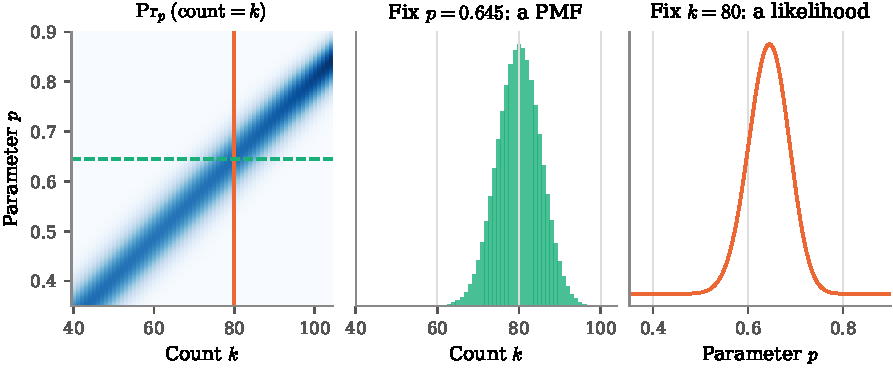
\includegraphics[width=\textwidth]{fig_likelihood_slices}
\caption{One function, two readings, for $124$ couples. Left: $\Pr_p(\text{count} = k)$ over counts $k$ (horizontal) and parameters $p$ (vertical); darker is more probable. Middle: the slice along the dashed aqua line, $p = 0.645$, a PMF over $k$ that sums to $1$. Right: the slice along the orange line, the observed $k = 80$, which is the likelihood; it peaks at $80/124 = 0.645$. The likelihood of the full sequence of $124$ turns is this curve divided by the constant $\binom{124}{80}$, which doesn't change where it peaks.}
\label{fig:likslices}
\end{figure}

\begin{pitfall}[the likelihood is not a distribution for $\theta$]
The likelihood curve in \cref{fig:likslices} looks like a density for $p$, and it isn't one.
The curve drawn there (the version for the count) has area $1/125$, not $1$, and the sequence likelihood $p^{80}(1 - p)^{44}$ has area $1.0 \times 10^{-36}$; nothing in the construction makes the area mean anything: rescale it by any constant and every comparison it supports is unchanged.
Until \cref{ch:bayes-intro}, $p$ is a fixed unknown number, not a random variable, so `the probability that $p$ is between $0.6$ and $0.7$' has no meaning here.
The likelihood is a plausibility ranking of candidate truths by how well they predicted your data.
This is why the right of \cref{fig:probstat} in \cref{ch:kiss}, which is this kind of curve for the drug data scaled to peak at $1$, has no vertical scale that could be read as a probability.
That chapter is where the parameter gets a distribution, and the likelihood is one of its two ingredients.
\end{pitfall}

\begin{worked}[the likelihoods of the two discrete families]
\begin{itemize}
\item \textbf{Bernoulli.} For $\Xton \iid \Bern(p)$, $E = \{0, 1\}$ and $\Theta = (0, 1)$. The PMF can be written in one line as $p_p(x) = p^x (1 - p)^{1 - x}$, which is $p$ at $x = 1$ and $1 - p$ at $x = 0$. Then
\[
L(x_1, \ldots, x_n; p) = \prod_{i=1}^n p^{x_i}(1 - p)^{1 - x_i} = p^{\sum_i x_i}(1 - p)^{n - \sum_i x_i}.
\]
The data enter only through the number of ones, $\sum_i x_i$.
\item \textbf{Poisson.} For $\Xton \iid \Pois(\lambda)$, $E = \{0, 1, 2, \ldots\}$ and $\Theta = (0, \infty)$:
\[
L(x_1, \ldots, x_n; \lambda) = \prod_{i=1}^n e^{-\lambda}\frac{\lambda^{x_i}}{x_i!} = e^{-n\lambda}\frac{\lambda^{\sum_i x_i}}{x_1! \cdots x_n!}.
\]
For the siblings data of \cref{ch:models}, modeled as $X_i - 1 \sim \Pois(\lambda)$, the $24$ values of $x_i - 1$ add up to $24$, and the likelihood is $e^{-24\lambda}\lambda^{24}$ divided by a constant that doesn't involve $\lambda$.
\end{itemize}
\end{worked}

Three properties of a likelihood follow straight from the product.

\begin{itemize}
\item \textbf{Order doesn't matter.} A product can be taken in any order, so the likelihood of $(1, 2, 3)$ is the likelihood of $(2, 3, 1)$. For the Bernoulli and Poisson families it depends on the data only through their sum, up to a factor that does not involve the parameter; the sum is the sufficient statistic of \cref{ch:estimators}: the likelihood never looks at anything else in the data.
\item \textbf{It updates one observation at a time.} If $L_n$ is the likelihood after $n$ observations, then $L_{n+1}(\theta) = L_n(\theta) \cdot p_\theta(x_{n+1})$. For Poisson data $1, 2$ the likelihood is $e^{-2\lambda}\lambda^3/2$; a third observation $3$ multiplies it by $e^{-\lambda}\lambda^3/6$, giving $e^{-3\lambda}\lambda^6/12$ (\cref{ex:lik-poisson-update}).
\item \textbf{It is as smooth in $\theta$ as the PMF is.} If each $p_\theta(x)$ is a continuous function of $\theta$, so is the product. A discrete model can have a perfectly smooth likelihood: the data are discrete, the parameter is not.
\end{itemize}

\section{The likelihood of a continuous model}
\label{sec:lik-continuous}

For continuous data the probability of observing exactly $x_1, \ldots, x_n$ is $0$ under every candidate, which would make every likelihood $0$ and rank nothing.
The fix is to use densities.

\begin{definition}[Likelihood, continuous model]
\label{def:likelihood-continuous}
Let $(E, (\Pr_\theta)_{\theta \in \Theta})$ be a statistical model for $\Xton$ i.i.d., where each $\Pr_\theta$ has a density $f_\theta$ \toolkit{sec:math-density}.
The \textbf{likelihood} of the model is
\begin{align*}
L_n : E^n \times \Theta &\to \real \\
(x_1, \ldots, x_n; \theta) &\mapsto \prod_{i=1}^n f_\theta(x_i).
\end{align*}
\end{definition}

\begin{inwords}
\textbf{In words.} The same recipe as for a discrete model, with each observation contributing the height of its density instead of its probability. A candidate whose density is high where your data fell scores well; one whose density is low there scores badly.
\par\smallskip
\textbf{For the kiss data.} The kiss data are discrete, so the discrete definition applies and this one doesn't. The two definitions are one idea, and from here on the chapter writes $p_\theta$ for either a PMF or a density.
\end{inwords}

\begin{intuition}[why the density is enough]
A recorded measurement is never exact.
A subway gap written down as $5$ minutes was somewhere near $5$, say within $h/2$ of it for a small $h$.
The probability of that is the area of a thin strip under the density, about $f_\lambda(5)\cdot h$.
Compare two candidate rates, and the $h$ cancels:
\[
\frac{\Pr_{\lambda_1}(\text{gap within } h/2 \text{ of } 5)}{\Pr_{\lambda_2}(\text{gap within } h/2 \text{ of } 5)} \approx \frac{f_{\lambda_1}(5)\, h}{f_{\lambda_2}(5)\, h} = \frac{f_{\lambda_1}(5)}{f_{\lambda_2}(5)}.
\]
\Cref{fig:densitystrip} shows the ratio of strip probabilities settling at the ratio of densities as the strip narrows.
Every use of a likelihood is a comparison between parameters, so the density is all it needs.
\end{intuition}

\begin{figure}[htbp]
\centering
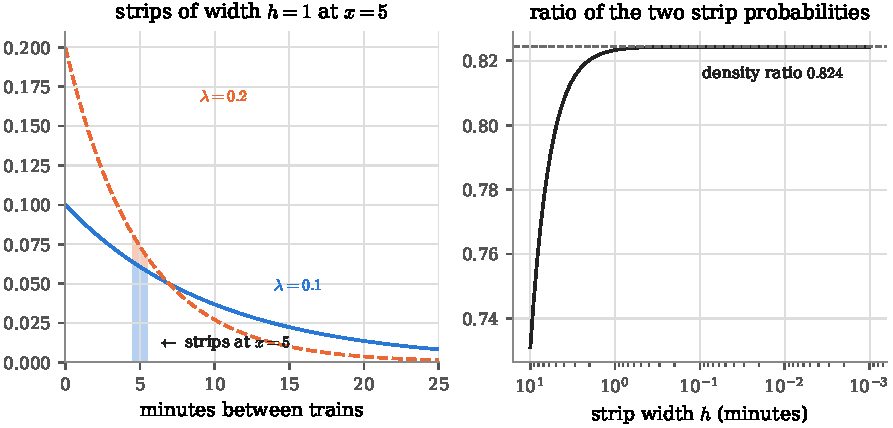
\includegraphics[width=\textwidth]{fig_density_strip}
\caption{Why a density can stand in for a probability. Left: the $\Expo(0.1)$ and $\Expo(0.2)$ densities, with the probabilities of a gap within $\frac12$ minute of $5$ shown as strips; the $\Expo(0.1)$ strip is blue, and the taller $\Expo(0.2)$ strip contains it, its extra height in orange. Right: the ratio of the two strip probabilities as the width $h$ shrinks; it settles at the ratio of the densities, $f_{0.1}(5)/f_{0.2}(5) = 0.824$.}
\label{fig:densitystrip}
\end{figure}

\begin{worked}[the likelihoods of the continuous families]
\begin{itemize}
\item \textbf{Gaussian.} For $\Xton \iid \Gauss(\mu, \sigma^2)$, $E = \real$ and $\Theta = \real \times (0, \infty)$:
\[
\begin{aligned}
L(x_1, \ldots, x_n; \mu, \sigma^2) &= \prod_{i=1}^n \frac{1}{\sigma\sqrt{2\pi}}\exp\left(-\frac{(x_i - \mu)^2}{2\sigma^2}\right)\\
&= \frac{1}{(\sigma\sqrt{2\pi})^n}\exp\left(-\frac{1}{2\sigma^2}\sum_{i=1}^n (x_i - \mu)^2\right).
\end{aligned}
\]
\item \textbf{Exponential.} For $\Xton \iid \Expo(\lambda)$, $E = (0, \infty)$ and $\Theta = (0, \infty)$. The density is $f_\lambda(x) = \lambda e^{-\lambda x}\ind(x > 0)$, so
\[
L(x_1, \ldots, x_n; \lambda) = \lambda^n e^{-\lambda \sum_i x_i} \prod_{i=1}^n \ind(x_i > 0) = \lambda^n e^{-\lambda \sum_i x_i}\, \ind\big(\min_i x_i > 0\big).
\]
The product of indicators is $1$ exactly when every $x_i$ is positive, which is when the smallest one is \toolkit{sec:math-indicator}. The indicator doesn't involve $\lambda$, and data from the model are always positive, so it is usually dropped: $L(\lambda) = \lambda^n e^{-\lambda\sum_i x_i}$.
\item \textbf{Uniform.} For $\Xton \iid \Unif([0, \theta])$, $E = [0, \infty)$ and $\Theta = (0, \infty)$. The density is $f_\theta(x) = \frac1\theta \ind(0 \leq x \leq \theta)$, so
\[
L(x_1, \ldots, x_n; \theta) = \frac{1}{\theta^n}\prod_{i=1}^n \ind(0 \leq x_i \leq \theta) = \frac{1}{\theta^n}\,\ind\big(\min_i x_i \geq 0\big)\,\ind\big(\max_i x_i \leq \theta\big).
\]
Every $x_i \leq \theta$ holds exactly when the largest does. Here the indicator involving the maximum \textit{does} depend on $\theta$, and it cannot be dropped: it is what makes this likelihood unusual (\cref{sec:lik-families}). The other indicator doesn't involve $\theta$ and is dropped as before: $L(\theta) = \theta^{-n}\ind(\theta \geq \max_i x_i)$.
\item \textbf{Mixture of two Gaussians.} For the model of \cref{sec:models-gmm}, with weight $\pi$ and components $\Gauss(\mu_1, \sigma_1^2)$ and $\Gauss(\mu_2, \sigma_2^2)$, the density of one observation is a sum, and
\[
L = \prod_{i=1}^n \left( \frac{\pi}{\sigma_1\sqrt{2\pi}} e^{-(x_i - \mu_1)^2/(2\sigma_1^2)} + \frac{1 - \pi}{\sigma_2\sqrt{2\pi}} e^{-(x_i - \mu_2)^2/(2\sigma_2^2)} \right).
\]
A product of sums does not simplify, and that is the source of the trouble in \cref{sec:lik-em}.
\end{itemize}
\end{worked}

\begin{pitfall}[an indicator you drop must not involve the parameter]
Dropping a factor from a likelihood is safe exactly when the factor doesn't depend on $\theta$: it multiplies every candidate's score by the same number and changes no comparison.
The exponential's $\ind(\min_i x_i > 0)$ is such a factor.
The uniform's $\ind(\max_i x_i \leq \theta)$ is not, and dropping it leaves $\theta^{-n}$, which grows without bound as $\theta \to 0$: the best candidate would be one under which your data were impossible.
\end{pitfall}

\section{The maximum likelihood estimator}
\label{sec:lik-mle}

\begin{definition}[Maximum likelihood estimator]
\label{def:mle}
Let $\Xton$ be an i.i.d.\ sample from a statistical model $(E, (\Pr_\theta)_{\theta \in \Theta})$ with likelihood $L$.
The \textbf{maximum likelihood estimator} (MLE) of $\theta$ is
\[
\hat{\theta}_n^{\text{MLE}} = \operatorname*{argmax}_{\theta \in \Theta} L(X_1, \ldots, X_n; \theta),
\]
provided the maximum exists and is attained at a single point.
\end{definition}

\begin{inwords}
\textbf{In words.} Among all the candidate truths the model allows, pick the one under which the data you actually got were most probable. Before the data arrive, $\hat{\theta}_n^{\text{MLE}}$ is a random variable, a function of $\Xton$ like every estimator in \cref{ch:estimators}; once they arrive it is a number, the maximum likelihood estimate.
\par\smallskip
\textbf{For the kiss data.} $L(p) = p^{80}(1 - p)^{44}$ is largest at $p = 80/124 = 0.645$ (\cref{sec:lik-families} does the calculus), so the maximum likelihood estimate is the sample proportion. In general $\hat{p}^{\text{MLE}} = \bar{R}_n$, the estimator \cref{ch:kiss} started from because it was the obvious one. In models where no estimator is obvious, the same principle still produces one.
\end{inwords}

In practice you maximize the logarithm of the likelihood, the \textbf{log-likelihood}
\[
\ell_n(\theta) = \log L(X_1, \ldots, X_n; \theta) = \sum_{i=1}^n \log p_\theta(X_i).
\]
Because $\log$ is strictly increasing, $L$ and $\ell_n$ have their maximum at the same $\theta$ \toolkit{sec:math-explog}.
There are three reasons to prefer $\ell_n$.
It turns a product of $n$ factors into a sum of $n$ terms, and sums are easier to differentiate.
It keeps the numbers in a sane range: $L(0.645) = 9.4 \times 10^{-36}$ for the kiss data, and for a few thousand observations a likelihood is smaller than any number a computer stores, while $\ell_n(0.645) = -80.65$ is an ordinary number.
And $\frac1n\ell_n(\theta)$ is an average, which is what the Law of Large Numbers and the Central Limit Theorem know how to handle; \cref{ch:mle-properties} uses that.

\Cref{fig:kissloglik} shows both curves for the kiss data.
The likelihood is a narrow peak at $0.645$ on a scale of $10^{-36}$.
The log-likelihood is a smooth hill whose top is at the same place, flat there, and $5.30$ higher than its value at $p = \frac12$.

\begin{figure}[htbp]
\centering
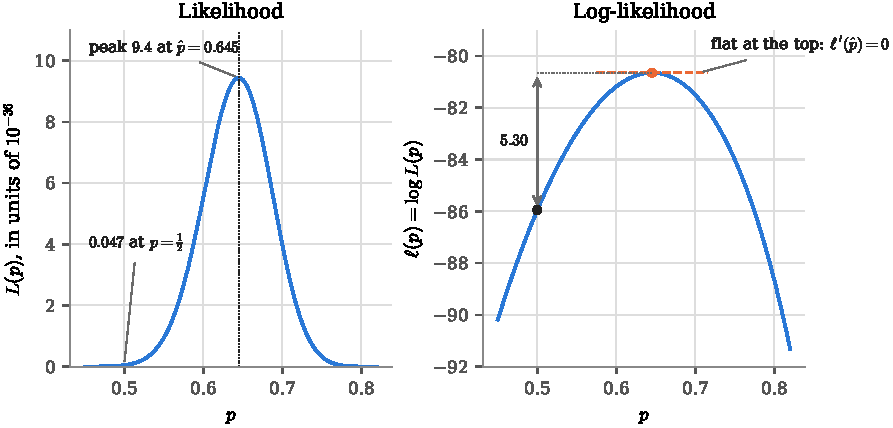
\includegraphics[width=\textwidth]{fig_kiss_loglik}
\caption{The kiss data. Left: the likelihood $L(p) = p^{80}(1 - p)^{44}$ in units of $10^{-36}$, with its peak $9.4$ at $\hat{p} = 0.645$ and the value $0.047$ at $p = \frac12$. Right: the log-likelihood $\ell(p) = 80\log p + 44\log(1 - p)$, concave, with its maximum $-80.65$ at $0.645$ where the tangent is flat, and the value $-85.95$ at $\frac12$; the gap, $5.30$, is $124$ times the KL divergence $0.0428$ of \cref{ch:distances}.}
\label{fig:kissloglik}
\end{figure}

\begin{sanitycheck}[The sharpness of the peak]
How sharply the log-likelihood curves down at its top should say something about how precisely the data pin down $p$: a flat top means many values of $p$ fit about equally well.
Check it.
For the kiss data $\ell(p) = 80\log p + 44\log(1 - p)$, so $\ell''(p) = -80/p^2 - 44/(1 - p)^2$, and at $\hat{p}$ this is $-n/(\hat{p}(1 - \hat{p})) = -541.7$.
Then $1/\sqrt{541.7} = 0.0430$, which is exactly the standard error $\sqrt{\hat{p}(1 - \hat{p})/n}$ of \cref{ch:confidence-intervals}, since $\ell''(\hat{p}) = -n/(\hat{p}(1 - \hat{p}))$.
For the subway data the same computation gives $\hat{\lambda}/\sqrt{n} = 0.020$, the standard error of \cref{ch:limit-tools}.
It is not a coincidence, and \cref{ch:mle-properties} proves it in general: the curvature of the log-likelihood at its peak estimates $n$ times the Fisher information, and one over its square root is the standard error of the MLE.
\end{sanitycheck}

\section{Finding a maximum}
\label{sec:lik-maximize}

The definition says `argmax', and an argmax has to be found.
Maximizing an arbitrary function is hard: it can have many hills, and a point where the slope is zero can be the top of a small hill, the bottom of a valley or neither.
The right of \cref{fig:concavevsnot} is $\theta \mapsto \prod_i (\theta - x_i)$ for five numbers $x_i$: four points with zero slope, and on the whole line no maximum at all.
The functions that are easy to maximize are the concave ones.

\begin{definition}[Concave and convex functions]
\label{def:concave}
A twice-differentiable function $h: \Theta \to \real$ on an interval $\Theta \subset \real$ is \textbf{concave} if $h''(\theta) \leq 0$ for every $\theta \in \Theta$, and \textbf{strictly concave} if $h''(\theta) < 0$ for every $\theta$.
(The `strictly' version here is stronger than the usual chord definition, which also allows $h'' = 0$ at isolated points, as for $-\theta^4$; it is the version this book uses.)
It is (strictly) \textbf{convex} if $-h$ is (strictly) concave, that is, $h'' \geq 0$ ($h'' > 0$).
\end{definition}

\begin{inwords}
\textbf{In words.} A concave function's slope never increases: it is a hill, or a straight line, never a valley. Every chord lies below the graph \toolkit{sec:math-convex}. On their natural domains, $-\theta^2$, $\sqrt{\theta}$, $\log\theta$ and $\sin\theta$ on $[0, \pi]$ are concave; $2\theta - 3$ is both concave and convex; $\theta^2$ and $e^\theta$ are convex.
\par\smallskip
\textbf{For the kiss data.} $\ell''(p) = -80/p^2 - 44/(1 - p)^2$ is negative for every $p \in (0, 1)$, so the kiss log-likelihood is strictly concave: one hill, no valleys, as the right of \cref{fig:kissloglik} shows.
\end{inwords}

\begin{proposition}[Maximizing a strictly concave function]
\label{prop:concave-max}
Let $h$ be strictly concave and differentiable on an open interval $\Theta$.
If $h'(\hat{\theta}) = 0$ at some $\hat{\theta} \in \Theta$, then $\hat{\theta}$ is the unique maximizer of $h$ on $\Theta$.
If $h'$ never vanishes, $h$ has no maximum on $\Theta$.
\end{proposition}

\optionalproof{Strict concavity makes the slope strictly decreasing, so it can cross zero at most once, and on each side of the crossing the function moves away from the top.}
\begin{proof}
Since $h'' < 0$, $h'$ is strictly decreasing.
If $h'(\hat{\theta}) = 0$, then $h' > 0$ to the left of $\hat{\theta}$ and $h' < 0$ to the right: $h$ increases up to $\hat{\theta}$ and decreases after, so $h(\theta) < h(\hat{\theta})$ for every $\theta \neq \hat{\theta}$.
At an interior maximizer the derivative must be $0$, since otherwise moving a little in the direction of the slope would increase $h$; so if $h'$ never vanishes there is no interior maximizer, and on an open interval there is no other kind.
\end{proof}

\begin{figure}[htbp]
\centering
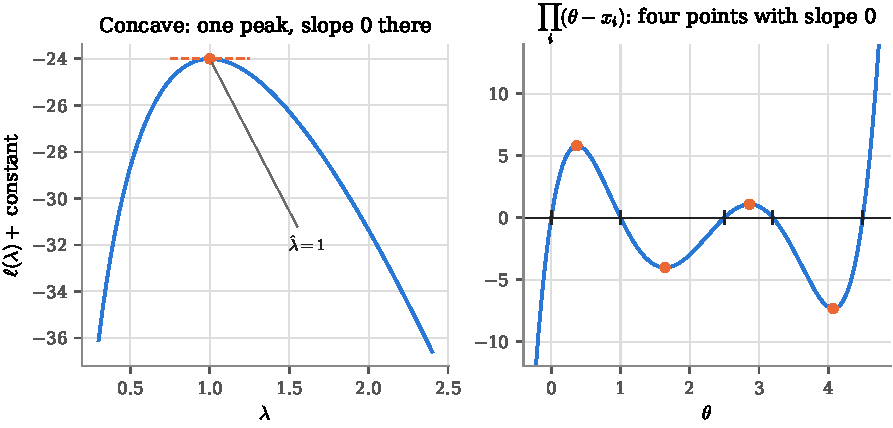
\includegraphics[width=\textwidth]{fig_concave_vs_not}
\caption{Easy and hard functions to maximize. Left: the Poisson log-likelihood of the siblings data, $-24\lambda + 24\log\lambda$ up to a constant, strictly concave with its single maximum at $\hat{\lambda} = 1$, where the slope is $0$. Right: $\prod_i (\theta - x_i)$ for the five values marked on the axis; four points have slope $0$ (dots), and setting the derivative to $0$ finds all four without saying which, if any, is a maximum.}
\label{fig:concavevsnot}
\end{figure}

So the recipe for a one-parameter model is: write $\ell_n$, check that it is strictly concave, solve $\ell_n'(\theta) = 0$.
The Bernoulli, Poisson and exponential log-likelihoods of \cref{sec:lik-families} pass the check; the Gaussian needs a two-step argument instead; the uniform fails it entirely.

For a parameter with several coordinates, $\theta = (\theta_1, \ldots, \theta_d)$, the derivative becomes the \textbf{gradient} $\nabla\ell_n(\theta)$, the vector of partial derivatives, and the second derivative becomes the \textbf{Hessian} $\nabla^2\ell_n(\theta)$, the $d \times d$ matrix of second partial derivatives \toolkit{sec:math-multivar}.
The first-order condition is $\nabla\ell_n(\hat{\theta}) = 0$, a system of $d$ equations.
A sufficient condition for strict concavity (on a $\Theta$ that contains the segment between any two of its points) is a negative definite Hessian at every $\theta$, which for $d = 2$ means its top-left entry is negative and its determinant positive.
Under it, the solution of $\nabla\ell_n = 0$, if there is one, is the unique maximizer, as in one dimension.
When there is no formula for the solution, numerical methods find it; for a concave $\ell_n$ they are reliable, and the subject of convex optimization is how to do it fast.

\section{Maximum likelihood estimators of the standard families}
\label{sec:lik-families}

\begin{worked}[Bernoulli: the kiss data]
For $\Xton \iid \Bern(p)$ with $S = \sum_i X_i$ ones,
\[
\ell_n(p) = S\log p + (n - S)\log(1 - p), \quad \ell_n'(p) = \frac{S}{p} - \frac{n - S}{1 - p}, \quad \ell_n''(p) = -\frac{S}{p^2} - \frac{n - S}{(1 - p)^2} < 0.
\]
Setting $\ell_n'(p) = 0$ gives $S(1 - p) = (n - S)p$, so $p = S/n$:
\[
\hat{p}^{\text{MLE}} = \bar{X}_n.
\]
(If $S = 0$ or $S = n$ there is no solution in $(0, 1)$; \cref{sec:lik-fail} deals with that.)
For the kiss data, $\hat{p} = 80/124 = 0.645$, the estimate of every earlier chapter.
\end{worked}

\begin{worked}[Poisson: the siblings data]
For $\Xton \iid \Pois(\lambda)$,
\[
\ell_n(\lambda) = -n\lambda + \Big(\sum_i X_i\Big)\log\lambda - \sum_i \log(X_i!), \quad \ell_n'(\lambda) = -n + \frac{\sum_i X_i}{\lambda}, \quad \ell_n''(\lambda) = -\frac{\sum_i X_i}{\lambda^2} < 0
\]
(when at least one $X_i$ is positive).
The first-order condition gives
\[
\hat{\lambda}^{\text{MLE}} = \bar{X}_n.
\]
For the siblings data, with $X_i - 1 \sim \Pois(\lambda)$, the sample mean of the $x_i - 1$ is $24/24 = 1$, so $\hat{\lambda} = 1.0$: the fit drawn in \cref{fig:siblings}, and the left of \cref{fig:concavevsnot}.
\end{worked}

\begin{worked}[exponential: the subway data]
For $\Xton \iid \Expo(\lambda)$,
\[
\ell_n(\lambda) = n\log\lambda - \lambda\sum_i X_i, \quad \ell_n'(\lambda) = \frac{n}{\lambda} - \sum_i X_i, \quad \ell_n''(\lambda) = -\frac{n}{\lambda^2} < 0,
\]
and
\[
\hat{\lambda}^{\text{MLE}} = \frac{n}{\sum_i X_i} = \frac{1}{\bar{X}_n}.
\]
For the $64$ subway gaps averaging $6.23$ minutes, $\hat{\lambda} = 0.1605$ per minute, the estimator of \cref{ch:limit-tools}.
\Cref{ch:estimators} showed it is biased upward, $\E[1/\bar{T}_n] = \frac{n}{n-1}\lambda$: a maximum likelihood estimator need not be unbiased.
\end{worked}

\begin{worked}[Gaussian: the boarding data]
For $\Xton \iid \Gauss(\mu, \sigma^2)$ the parameter has two coordinates, and
\[
\ell_n(\mu, \sigma^2) = -\frac{n}{2}\log(2\pi\sigma^2) - \frac{1}{2\sigma^2}\sum_{i=1}^n (X_i - \mu)^2.
\]
Maximize in $\mu$ first, for a fixed $\sigma^2$.
The only term involving $\mu$ is $-\frac{1}{2\sigma^2}\sum_i(X_i - \mu)^2$, and the split
\[
\sum_{i=1}^n (X_i - \mu)^2 = \sum_{i=1}^n (X_i - \bar{X}_n)^2 + n(\bar{X}_n - \mu)^2
\]
(write $X_i - \mu = (X_i - \bar{X}_n) + (\bar{X}_n - \mu)$, square, and note the cross terms add to $0$) shows it is largest at $\mu = \bar{X}_n$, whatever $\sigma^2$ is.
Now put $\mu = \bar{X}_n$ and maximize in $\sigma^2$.
With $D = \sum_i (X_i - \bar{X}_n)^2$, the function $-\frac{n}{2}\log\sigma^2 - D/(2\sigma^2)$ has derivative $-\frac{n}{2\sigma^2} + \frac{D}{2\sigma^4}$, positive for $\sigma^2 < D/n$ and negative after.
Chaining the two steps, for every $(\mu, \sigma^2)$,
\[
\ell_n(\mu, \sigma^2) \leq \ell_n(\bar{X}_n, \sigma^2) \leq \ell_n(\bar{X}_n, D/n),
\]
with equality only at $(\bar{X}_n, D/n)$, so
\[
\hat{\mu}^{\text{MLE}} = \bar{X}_n, \qquad \widehat{\sigma^2}^{\text{MLE}} = \frac1n\sum_{i=1}^n (X_i - \bar{X}_n)^2.
\]
At the maximum the gradient is $0$ and the Hessian is the diagonal matrix with entries $-n/\widehat{\sigma^2}$ and $-n/(2\widehat{\sigma^2}^2)$, negative definite.
(The log-likelihood is not concave in $\sigma^2$ everywhere, which is why the argument went one coordinate at a time instead of checking the Hessian at every point. It also needs $D > 0$: if every observation is the same number, the likelihood grows without bound as $\sigma^2 \to 0$.)

For the $72$ flights boarded rear to front, with mean $24.2$ minutes and standard deviation $s = 2.1$ (taken to be computed with $n - 1$, the usual convention), $\hat{\mu} = 24.2$ and $\widehat{\sigma^2} = \frac{71}{72} \times 2.1^2 = 4.35$.
\Cref{fig:gaussloglik} draws the log-likelihood surface.
\end{worked}

\begin{figure}[htbp]
\centering
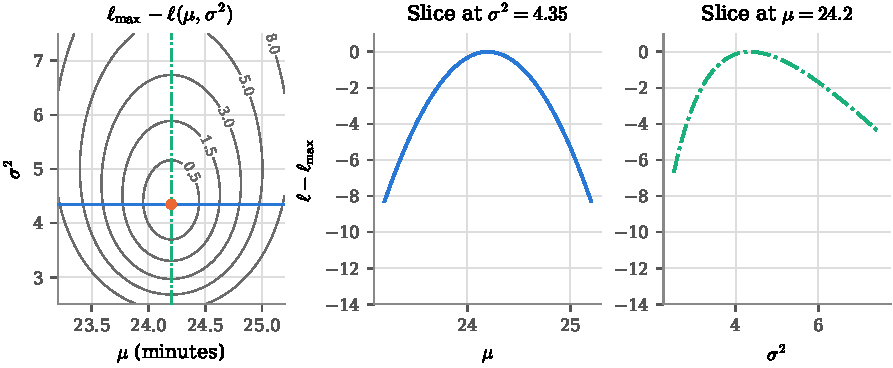
\includegraphics[width=\textwidth]{fig_gauss_loglik}
\caption{The Gaussian log-likelihood of the boarding data ($n = 72$, mean $24.2$, standard deviation $2.1$), measured from its maximum. Left: contours over $(\mu, \sigma^2)$, labeled by how far each lies below the maximum, with the maximum at $(24.2, 4.35)$ and the two slices drawn as lines (blue solid, aqua dash-dot). Middle: the slice at $\sigma^2 = 4.35$, symmetric in $\mu$. Right: the slice at $\mu = 24.2$, lopsided: variances above the maximum are penalized less than variances below it.}
\label{fig:gaussloglik}
\end{figure}

\begin{bridge}[$n$ or $n - 1$?]
The maximum likelihood estimator of the variance divides by $n$.
The sample variance you were taught divides by $n - 1$.
They differ by the factor $(n - 1)/n$, which is $0.986$ for the boarding data: $4.35$ against $4.41$.
\Cref{ch:estimators} showed that dividing by $n$ is biased low by exactly that factor and that dividing by $n - 1$ removes the bias; it also showed that removing the bias is not the same as minimizing the risk.
Maximum likelihood doesn't aim at unbiasedness, so it lands on $n$.
For large $n$ the difference is negligible, and every large-sample result in \cref{ch:mle-properties} holds for either.
\end{bridge}

\begin{bridge}[least squares is maximum likelihood]
The Gaussian log-likelihood contains $-\frac{1}{2\sigma^2}\sum_i (X_i - \mu)^2$, so maximizing it over $\mu$ is minimizing a sum of squared deviations.
The same is true when $\mu$ is replaced by a regression line $a + b x_i$: if the errors around the line are Gaussian with a common variance, the maximum likelihood estimates of $a$ and $b$ are the least squares estimates of an introductory regression course.
\Cref{ch:regression-uni} starts from that observation.
\end{bridge}

\begin{worked}[uniform: where calculus fails]
For $\Xton \iid \Unif([0, \theta])$ the likelihood is $L(\theta) = \theta^{-n}\ind(\theta \geq \max_i X_i)$.
Below the largest observation the likelihood is $0$ (a $\theta$ smaller than an observation makes that observation impossible). From the largest observation on it is $\theta^{-n}$, which decreases, with derivative $-n\theta^{-n-1}$, never $0$.
The maximum is at the jump:
\[
\hat{\theta}^{\text{MLE}} = \max_i X_i.
\]
\Cref{fig:uniformlik} draws it for five observations whose largest is $7.6$.
Setting the derivative to $0$ would have found only the flat stretch below $\max_i X_i$, where the likelihood is $0$; the recipe of \cref{sec:lik-maximize} assumes a smooth function with its maximum inside $\Theta$, and this likelihood is neither smooth at its maximum nor concave.
The estimator is also biased: the largest of $n$ draws always falls short of $\theta$, and $\E[\max_i X_i] = \frac{n}{n+1}\theta$ (\cref{ex:lik-uniform}). Multiplying by $\frac{n+1}{n}$ removes the bias.
\end{worked}

\begin{figure}[htbp]
\centering
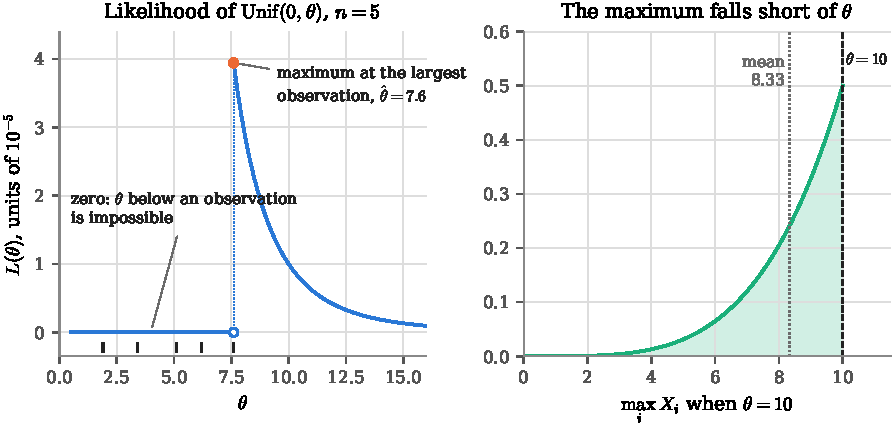
\includegraphics[width=\textwidth]{fig_uniform_likelihood}
\caption{Left: the likelihood of $\Unif([0, \theta])$ for five observations (ticks below the axis), zero until the largest observation, $7.6$, then $\theta^{-5}$, decreasing. The maximum is at the jump, where no derivative is zero. Right: the density $5m^4/10^5$ of the maximum of five draws when $\theta = 10$; it never exceeds $10$, and its mean is $8.33$.}
\label{fig:uniformlik}
\end{figure}

\begin{intuition}[the German tank problem]
The uniform model once estimated an enemy's tank production.
During the Second World War, Allied statisticians estimated German tank production from the serial numbers on captured tanks.
If serial numbers run $1, 2, \ldots, N$ and the captured ones are a random sample, $N$ plays the role of $\theta$, the largest serial number seen is the maximum likelihood estimate, and correcting it for the shortfall of the maximum gives a better one.
Their serial-number estimates, which refined this idea and used markings on several components (chassis, gearboxes, wheels), for three months, beside the figures from conventional intelligence and the German records found after the war:\footnote{R.~Ruggles and H.~Brodie, `An empirical approach to economic intelligence in World War II', \textit{Journal of the American Statistical Association} 42 (1947), 72--91.}
\begin{center}
\begin{tabular}{lrrr}
Month & Statistical estimate & Intelligence estimate & German records \\
\hline
June 1940 & 169 & 1{,}000 & 122 \\
June 1941 & 244 & 1{,}550 & 271 \\
August 1942 & 327 & 1{,}550 & 342
\end{tabular}
\end{center}
The model is crude (serial numbers are not quite a random sample), and its estimates were within $50$ tanks of the records while the intelligence estimates were off by a factor of about four to eight.
\end{intuition}

One more property makes maximum likelihood convenient: it doesn't care how the parameter is written.

\begin{proposition}[Invariance]
\label{prop:mle-invariance}
Let $g: \Theta \to g(\Theta)$ be one-to-one, and reparameterize the model by $\eta = g(\theta)$.
If $\hat{\theta}$ is the MLE of $\theta$, then $g(\hat{\theta})$ is the MLE of $\eta$.
\end{proposition}

\optionalproof{Reparameterizing relabels the candidates without changing any candidate's likelihood, so the winner is the same distribution under its new label.}
\begin{proof}
The candidate labeled $\eta$ in the new parameterization is the distribution $\Pr_{g^{-1}(\eta)}$, so its likelihood is $L(g^{-1}(\eta))$.
This is largest when $g^{-1}(\eta) = \hat{\theta}$, that is, at $\eta = g(\hat{\theta})$.
\end{proof}

For the subway data, the mean gap $\beta = 1/\lambda$ has MLE $1/\hat{\lambda} = \bar{X}_n = 6.23$ minutes.
For the boarding data, the standard deviation has MLE $\sqrt{4.35} = 2.09$ minutes.
Invariance does not carry unbiasedness along: $\bar{X}_n$ is unbiased for $\beta$ and $1/\bar{X}_n$ is biased for $\lambda$, though both are maximum likelihood estimators.

\section{When the maximum likelihood estimator fails to exist or isn't unique}
\label{sec:lik-fail}

\Cref{def:mle} said `provided the maximum exists and is attained at a single point'. Both can fail, in ordinary models.

\begin{pitfall}[three ways the definition can fail]
\begin{itemize}
\item \textbf{No maximum: the data sit on the boundary.} If every observation in a Bernoulli sample is $0$ ($S = 0$), then $L(p) = (1 - p)^n$ increases as $p$ decreases and has no maximum on $\Theta = (0, 1)$: the supremum is at $p = 0$, which the model excludes. For the kiss data this can't happen in practice (under $p = 0.645$ its probability is $0.355^{124}$), but for $n = 5$ observations of an outcome with $p = 0.1$ it happens $59\%$ of the time. The usual repair is to allow $p \in [0, 1]$, and then $\hat{p} = 0$.
\item \textbf{More than one maximum.} For $\Xton \iid \Unif([\theta, \theta + 1])$, $L(\theta) = \ind(\theta \leq \min_i X_i)\,\ind(\theta + 1 \geq \max_i X_i)$, which equals $1$ on the whole interval $[\max_i X_i - 1, \min_i X_i]$ and $0$ elsewhere. Every point of that interval is a maximizer (\cref{ex:lik-unif-shift}).
\item \textbf{An unbounded likelihood.} In the mixture of two Gaussians with unknown variances, put $\mu_1 = x_1$ and let $\sigma_1 \to 0$. The first factor of the likelihood contains $\pi/(\sigma_1\sqrt{2\pi})$, which goes to infinity, while every other factor stays above $(1 - \pi)$ times the second component's density at its point, which is positive. The likelihood is unbounded: a component of zero width sitting on one data point `explains' that point infinitely well. The maximum likelihood estimator of a mixture with free variances does not exist, and what is computed in practice is the best local maximum away from these spikes.
\end{itemize}
\end{pitfall}

\section{No formula: mixtures and the EM algorithm}
\label{sec:lik-em}

The left of \cref{fig:emfaithful} is a histogram of the $272$ waiting times, in minutes, between eruptions of the Old Faithful geyser in Yellowstone National Park.\footnote{The version of the data distributed with W.~H\"ardle, \textit{Smoothing Techniques} (Springer, 1991); A.~Azzalini and A.~W.~Bowman, `A look at some data on the Old Faithful geyser', \textit{Applied Statistics} 39 (1990), 357--365, analyze a longer record.}
It has two humps, one near $55$ minutes and one near $80$, and a single Gaussian (orange) fits it badly.
A mixture of two Gaussians is the natural model: each wait comes from a short-wait regime or a long-wait regime, and you don't get to see which.

The log-likelihood of the mixture,
\[
\ell_n = \sum_{i=1}^n \log\Big( \pi\, f_{\mu_1, \sigma_1^2}(X_i) + (1 - \pi)\, f_{\mu_2, \sigma_2^2}(X_i) \Big),
\]
has the log of a sum in every term, and setting its gradient to $0$ gives five equations with no closed-form solution.
The \textbf{EM algorithm} (expectation-maximization, given its general form and its name in 1977 and still in everyday use) gets around this with one idea: pretend you know which regime each observation came from.

\subsection*{The complete data}

Recall the generative story of \cref{sec:models-gmm}: draw $Z_i \sim \Bern(\pi)$; if $Z_i = 1$, draw $X_i$ from component $1$, otherwise from component $2$.
If you observed the labels $Z_i$ along with the $X_i$, the log-likelihood of the \textit{complete data} $(X_i, Z_i)$ would split:
\[
\ell_n^{\text{comp}} = \sum_{i=1}^n \Big[ Z_i\big(\log\pi + \log f_{\mu_1, \sigma_1^2}(X_i)\big) + (1 - Z_i)\big(\log(1 - \pi) + \log f_{\mu_2, \sigma_2^2}(X_i)\big) \Big].
\]
There is no log of a sum: each observation contributes to exactly one component.
Maximizing it is two separate Gaussian fits and one Bernoulli fit, each done in \cref{sec:lik-families}: $\hat{\pi}$ is the share of observations labeled $1$, and $\hat{\mu}_1$, $\hat{\sigma}_1^2$ are the mean and divide-by-$n$ variance of the observations labeled $1$ (and likewise for component $2$).

\subsection*{The E step: guess the labels}

You don't observe the $Z_i$.
The best guess for $Z_i$ given $X_i$, under the current parameter values, is its conditional expectation, which is the probability that $X_i$ came from component $1$.
By Bayes' formula,
\[
w_i = \E[Z_i \mid X_i] = \Pr(Z_i = 1 \mid X_i) = \frac{\pi\, f_{\mu_1, \sigma_1^2}(X_i)}{\pi\, f_{\mu_1, \sigma_1^2}(X_i) + (1 - \pi)\, f_{\mu_2, \sigma_2^2}(X_i)} \in (0, 1).
\]
A wait of $50$ minutes gets $w_i$ close to $1$; a wait of $85$ gets $w_i$ close to $0$; a wait of $67$, between the humps, gets something in the middle.
Guessing $Z_i \approx \E[Z_i] = \pi$, the same for every observation, would ignore the data entirely; conditioning on $X_i$ is what makes the guess useful.

\subsection*{The M step: fit as if the guesses were labels}

Replace each $Z_i$ in $\ell_n^{\text{comp}}$ by $w_i$ and maximize.
This is legitimate because $\ell_n^{\text{comp}}$ is linear in each $Z_i$, so its expectation given the data, under the current parameter values, is $\ell_n^{\text{comp}}$ with each $Z_i$ replaced by $w_i$.
The same calculus as before, with weights, gives
\[
\hat{\pi} = \frac1n\sum_i w_i, \quad \hat{\mu}_1 = \frac{\sum_i w_i X_i}{\sum_i w_i}, \quad \hat{\sigma}_1^2 = \frac{\sum_i w_i (X_i - \hat{\mu}_1)^2}{\sum_i w_i},
\]
and the same for component $2$ with weights $1 - w_i$ (\cref{ex:lik-em-mstep}).
Each observation is split between the components in proportion to how likely it is to belong to each.

\begin{worked}[the EM algorithm]
\begin{enumerate}[nosep]
\item Start from some values of $\pi, \mu_1, \mu_2, \sigma_1^2, \sigma_2^2$.
\item \textbf{E step:} compute $w_i$ for every observation from the current values.
\item \textbf{M step:} update all five parameters by the weighted formulas.
\item Repeat steps 2 and 3 until the parameters stop changing.
\end{enumerate}
For Old Faithful, starting from means $50$ and $70$, both standard deviations $10$ and $\pi = \frac12$, the algorithm settles on weight $0.36$ for $\Gauss(54.6, 5.87^2)$ and $0.64$ for $\Gauss(80.1, 5.87^2)$: about a third of the waits are short, averaging $55$ minutes, and the rest are long, averaging $80$. The fitted mixture is the blue curve in \cref{fig:emfaithful}. Its log-likelihood is $-1034.0$, against $-1095.3$ for the best single Gaussian.
\end{worked}

\begin{figure}[htbp]
\centering
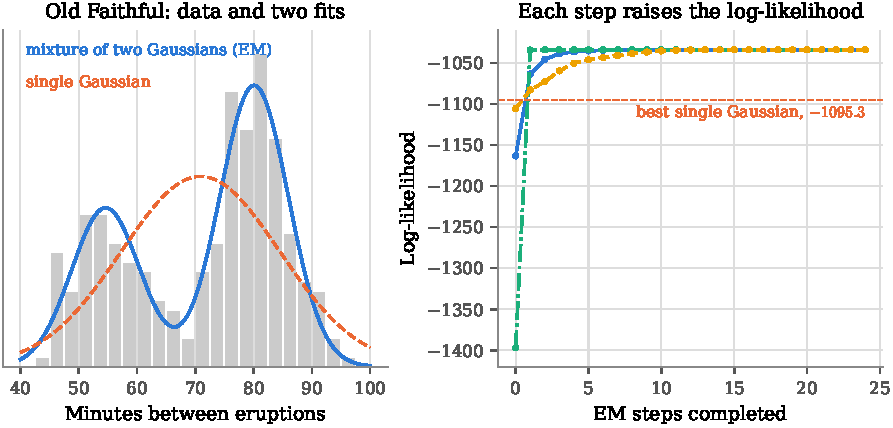
\includegraphics[width=\textwidth]{fig_em_faithful}
\caption{The EM algorithm on the $272$ waiting times between eruptions of Old Faithful. Left: the histogram, the best single Gaussian (orange, dashed) and the two-component mixture fitted by EM (blue): weight $0.36$ on $\Gauss(54.6, 5.87^2)$ and $0.64$ on $\Gauss(80.1, 5.87^2)$. Right: the log-likelihood at the start and after each EM step, from three starting points: means $50$ and $70$ (blue, solid), $40$ and $95$ (aqua, dash-dot), $65$ and $75$ (yellow, dashed). It never decreases, and all three runs reach $-1034.0$, well above the single Gaussian's $-1095.3$ (orange line).}
\label{fig:emfaithful}
\end{figure}

The right of \cref{fig:emfaithful} shows the property that makes EM trustworthy as far as it goes: every step raises the log-likelihood or leaves it unchanged.
That fact is proved in \cref{sec:proof-em} of \cref{app:proofs}, with an argument that uses the nonnegativity of the KL divergence; nothing later in the book depends on it.
What it does not guarantee is that EM reaches the highest point.
It climbs whatever hill it starts near, which may be a local maximum or one of the spikes of \cref{sec:lik-fail}.
In practice EM is run from several starting points and the run with the largest log-likelihood is kept.
EM is guaranteed to climb, not to reach the top: the results that guarantee it reaches the maximum likelihood estimate assume a starting point close enough to it, or well-separated components.

\begin{pitfall}[which component is which]
EM's labels `component $1$' and `component $2$' mean nothing.
Start it with the means the other way round and it returns the same fit with the labels swapped: weight $0.64$ on $\Gauss(80.1, 5.87^2)$ and $0.36$ on $\Gauss(54.6, 5.87^2)$.
Both have the same likelihood, since they are the same distribution.
This is the label switching of \cref{sec:models-gmm}: the mixture's parameter is identifiable only up to relabeling, so every peak of its likelihood has a twin with the labels swapped.
\end{pitfall}

\section{What comes next}
\label{sec:lik-next}

This chapter defined the maximum likelihood estimator and computed it.
\Cref{ch:mle-properties} asks how good it is, and answers with three results that hold for every well-behaved model at once.
It is consistent, by the argument \cref{fig:klestimate} drew: the average log-likelihood converges to a function maximized at the truth.
It is asymptotically normal, by the Central Limit Theorem applied to the derivative of the log-likelihood.
And its asymptotic variance is one over the Fisher information, the curvature that the sanity check of \cref{sec:lik-mle} found matching the standard errors of earlier chapters.
\Cref{ch:mom-mestimation} generalizes in two directions: the method of moments, an older and simpler recipe that often gives the same answer, and M-estimation, which maximizes or minimizes averages other than the log-likelihood.

\section{Summary}
\label{sec:lik-summary}

\begin{itemize}[nosep]
\item The likelihood $L(\theta) = \prod_i p_\theta(x_i)$ (PMFs) or $\prod_i f_\theta(x_i)$ (densities) is the probability or density of the observed data under each candidate $\theta$: the joint PMF read with the data fixed and the parameter varying. It is not a distribution for $\theta$; only ratios of likelihoods mean something. Kiss data: $L(p) = p^{80}(1 - p)^{44}$, $200$ times larger at $0.645$ than at $\frac12$.
\item A density works in place of a probability because a recorded value stands for a small interval, whose width cancels in every comparison between parameters.
\item The likelihood ignores the order of the data, updates one observation at a time, and is as smooth in $\theta$ as the PMF or density. Factors that don't involve $\theta$ (the exponential's indicator) can be dropped; factors that do (the uniform's $\ind(\theta \geq \max_i x_i)$) cannot.
\item MLE: $\hat{\theta}^{\text{MLE}} = \operatorname{argmax}_\theta L = \operatorname{argmax}_\theta \ell_n$, with $\ell_n = \sum_i \log p_\theta(X_i)$. If $\ell_n$ is strictly concave, the solution of $\ell_n' = 0$ (or $\nabla\ell_n = 0$) is the unique maximizer; in several dimensions, a negative definite Hessian everywhere is enough for strict concavity.
\item Bernoulli $\bar{X}_n$ ($0.645$ for the kiss data); Poisson $\bar{X}_n$ ($1.0$ for the siblings); exponential $1/\bar{X}_n$ ($0.1605$ per minute for the subway); Gaussian $\bar{X}_n$ and $\frac1n\sum(X_i - \bar{X}_n)^2$ ($24.2$ and $4.35$ for boarding); uniform $\max_i X_i$, found at a jump rather than where a derivative vanishes, and biased low by the factor $n/(n+1)$.
\item The curvature of the log-likelihood at its peak gives the standard error: $1/\sqrt{541.7} = 0.043$ for the kiss data.
\item Invariance: the MLE of $g(\theta)$ is $g(\hat{\theta})$ for one-to-one $g$. Unbiasedness is not invariant.
\item The MLE can fail to exist (all-zero Bernoulli data on $(0, 1)$; mixtures with free variances, whose likelihood is unbounded) or be non-unique ($\Unif([\theta, \theta+1])$).
\item EM for mixtures: E step $w_i = \Pr(Z_i = 1 \mid X_i)$ by Bayes' formula; M step, weighted proportions, means and variances. No step lowers the log-likelihood; it can stop at a local maximum, so run it from several starts. Old Faithful: weight $0.36$ on mean $54.6$, $0.64$ on mean $80.1$, log-likelihood $-1034.0$ against $-1095.3$ for one Gaussian.
\end{itemize}

\section{Exercises}
\label{sec:lik-exercises}

\begin{exercise}
\label{ex:lik-poisson-update}
Let $\Xton \iid \Pois(\lambda)$. You observe $X_1 = 1$, $X_2 = 2$. Compute $L_2(1, 2; \lambda)$. A third observation $X_3 = 3$ arrives: compute $L_3(1, 2, 3; \lambda)$ in two ways, from the definition and by updating $L_2$. Then compute $L_3(2, 3, 1; \lambda)$ and explain why it is the same.
\end{exercise}
\begin{solution}
$L_2(1, 2; \lambda) = e^{-\lambda}\frac{\lambda^1}{1!} \cdot e^{-\lambda}\frac{\lambda^2}{2!} = e^{-2\lambda}\frac{\lambda^3}{2}$. From the definition, $L_3(1, 2, 3; \lambda) = e^{-3\lambda}\frac{\lambda^{1+2+3}}{1!\,2!\,3!} = e^{-3\lambda}\frac{\lambda^6}{12}$. By updating, $L_3 = L_2 \cdot e^{-\lambda}\frac{\lambda^3}{3!} = e^{-2\lambda}\frac{\lambda^3}{2}\cdot e^{-\lambda}\frac{\lambda^3}{6} = e^{-3\lambda}\frac{\lambda^6}{12}$. $L_3(2, 3, 1; \lambda)$ is the same product with the factors in a different order, so it is also $e^{-3\lambda}\lambda^6/12$: the likelihood of i.i.d.\ data does not depend on the order of the observations. The MLE from the three observations is $\bar{X}_3 = 2$.
\end{solution}

\begin{exercise}
\label{ex:lik-continuity}
Let $(\mathbb{Z}, (\Pr_\theta)_{\theta \in \real})$ be a discrete model whose PMF $p_\theta(x)$ is a continuous function of $\theta$ for each fixed $x$. True or false: for fixed data $x_1, \ldots, x_n$, the likelihood $\theta \mapsto L_n(x_1, \ldots, x_n; \theta)$ is continuous. Give a discrete model with a smooth likelihood.
\end{exercise}
\begin{solution}
True. $L_n(\theta) = \prod_{i=1}^n p_\theta(x_i)$ is a product of $n$ continuous functions of $\theta$, and a product of continuous functions is continuous. The Bernoulli likelihood $p^{S}(1 - p)^{n - S}$ is a polynomial in $p$, as smooth as a function can be, although the data take only the values $0$ and $1$. The Poisson likelihood $e^{-n\lambda}\lambda^{\sum x_i}/\prod x_i!$ is another.
\end{solution}

\begin{exercise}
\label{ex:lik-gauss-known-mean}
Let $\Xton \iid \Gauss(0, \sigma^2)$ with $\sigma^2 > 0$ unknown. Find the MLE of $\sigma^2$, check that the log-likelihood has a unique maximum, and use invariance to find the MLE of $\sigma$.
\end{exercise}
\begin{solution}
$\ell_n(\sigma^2) = -\frac{n}{2}\log(2\pi\sigma^2) - \frac{1}{2\sigma^2}\sum_i X_i^2$. With $v = \sigma^2$ and $Q = \sum_i X_i^2$, $\ell_n'(v) = -\frac{n}{2v} + \frac{Q}{2v^2} = \frac{Q - nv}{2v^2}$, positive for $v < Q/n$ and negative for $v > Q/n$, so the unique maximizer is $\widehat{\sigma^2} = \frac1n\sum_i X_i^2$. (The log-likelihood is not concave in $v$ for all $v$, which is why the sign of the derivative is used instead of the second derivative.) It is unbiased here, since the mean is known: $\E[X_i^2] = \sigma^2$. By invariance, $\hat{\sigma} = \sqrt{\frac1n\sum_i X_i^2}$.
\end{solution}

\begin{exercise}
\label{ex:lik-uniform}
Let $\Xton \iid \Unif([0, \theta])$ and $M = \max_i X_i$. Show that $\Pr(M \leq m) = (m/\theta)^n$ for $0 \leq m \leq \theta$, find the density of $M$, and show that $\E[M] = \frac{n}{n+1}\theta$. Which multiple of $M$ is unbiased?
\end{exercise}
\begin{solution}
$M \leq m$ exactly when every $X_i \leq m$, and by independence $\Pr(M \leq m) = \prod_i \Pr(X_i \leq m) = (m/\theta)^n$. Differentiating, $M$ has density $n m^{n-1}/\theta^n$ on $[0, \theta]$. Then $\E[M] = \int_0^\theta m \cdot \frac{n m^{n-1}}{\theta^n}\, \mathrm{d}m = \frac{n}{\theta^n}\cdot\frac{\theta^{n+1}}{n+1} = \frac{n}{n+1}\theta$. So $\frac{n+1}{n}M$ is unbiased. For the five observations of \cref{fig:uniformlik}, $\frac65 \times 7.6 = 9.12$. The bias of $M$ is $-\theta/(n+1)$, of order $1/n$, and its standard deviation is also of order $1/n$, not $1/\sqrt{n}$: this model is not one of the regular models whose large-sample theory \cref{ch:mle-properties} develops.
\end{solution}

\begin{exercise}
\label{ex:lik-unif-shift}
Let $\Xton \iid \Unif([\theta, \theta + 1])$ with $\theta \in \real$. Write the likelihood and show that every $\theta$ in $[\max_i X_i - 1, \min_i X_i]$ maximizes it. Why is that interval never empty?
\end{exercise}
\begin{solution}
Each density is $\ind(\theta \leq x_i \leq \theta + 1)$, so $L(\theta) = \prod_i \ind(\theta \leq x_i)\ind(x_i \leq \theta + 1) = \ind(\theta \leq \min_i x_i)\,\ind(\theta \geq \max_i x_i - 1)$. It is $1$ on $[\max_i x_i - 1, \min_i x_i]$ and $0$ elsewhere, so every point of that interval maximizes it and the MLE is not unique. The interval is nonempty because all the data lie in an interval of length $1$, $[\theta^*, \theta^* + 1]$, so $\max_i x_i - \min_i x_i \leq 1$. Its midpoint is a sensible choice of estimate, but the likelihood alone doesn't pick it.
\end{solution}

\begin{exercise}
\label{ex:lik-geometric}
A basketball player takes shots until the first one goes in; the number of shots is $X \sim \text{Geom}(p)$, with $\Pr(X = k) = (1 - p)^{k-1}p$ for $k = 1, 2, \ldots$. Over $n$ independent rounds the numbers of shots are $\Xton$. Find the MLE of $p$, and evaluate it for rounds of $3$, $1$, $2$, $5$ and $1$ shots.
\end{exercise}
\begin{solution}
$\ell_n(p) = \sum_i\big[(X_i - 1)\log(1 - p) + \log p\big] = (S - n)\log(1 - p) + n\log p$ with $S = \sum_i X_i$. $\ell_n'(p) = -\frac{S - n}{1 - p} + \frac{n}{p} = 0$ gives $n(1 - p) = (S - n)p$, so $p = n/S$: $\hat{p} = 1/\bar{X}_n$. $\ell_n''(p) = -\frac{S - n}{(1-p)^2} - \frac{n}{p^2} < 0$, so this is the unique maximum. For the data, $S = 12$ and $n = 5$, so $\hat{p} = 5/12 = 0.417$: five makes in twelve shots.
\end{solution}

\begin{exercise}
\label{ex:lik-shifted-expo}
Let $\Xton$ be i.i.d.\ with density $f_a(x) = e^{-(x - a)}\ind(x \geq a)$, an exponential shifted to start at an unknown $a \in \real$. Find the MLE of $a$.
\end{exercise}
\begin{solution}
$L(a) = \prod_i e^{-(x_i - a)}\ind(x_i \geq a) = e^{na - \sum_i x_i}\,\ind(a \leq \min_i x_i)$. For $a \leq \min_i x_i$ this is increasing in $a$; beyond, it is $0$. So $\hat{a} = \min_i X_i$, found at the jump, as for the uniform. Again no derivative vanishes where $L > 0$, and again the estimator is biased: $\min_i X_i - a \sim \Expo(n)$, so $\E[\hat{a}] = a + 1/n$.
\end{solution}

\begin{exercise}
\label{ex:lik-laplace}
Let $\Xton$ be i.i.d.\ with the Laplace density $f_m(x) = \frac12 e^{-\abs{x - m}}$, $m \in \real$, and $n$ odd. Show that the MLE of $m$ is the sample median.
\end{exercise}
\begin{solution}
$\ell_n(m) = -n\log 2 - \sum_i\abs{X_i - m}$, so maximizing it is minimizing $g(m) = \sum_i \abs{X_i - m}$. Away from the data points, $g'(m) = (\text{number of } X_i < m) - (\text{number of } X_i > m)$, which is negative when fewer than half the observations lie below $m$ and positive when more than half do. With $n$ odd, $g$ decreases until the middle observation and increases after it, so the minimizer is the sample median. The Gaussian's squared deviations give the mean; the Laplace's absolute deviations give the median. \Cref{ch:mom-mestimation} takes this up as M-estimation.
\end{solution}

\begin{exercise}
\label{ex:lik-em-mstep}
Derive the M-step formulas for $\pi$ and $\mu_1$: maximize $\sum_i [w_i(\log\pi + \log f_{\mu_1,\sigma_1^2}(X_i)) + (1 - w_i)(\log(1-\pi) + \log f_{\mu_2,\sigma_2^2}(X_i))]$ over $\pi$ and over $\mu_1$.
\end{exercise}
\begin{solution}
The terms involving $\pi$ are $\big(\sum_i w_i\big)\log\pi + \big(\sum_i (1 - w_i)\big)\log(1 - \pi)$: the Bernoulli log-likelihood with $\sum_i w_i$ `successes' out of $n$, maximized at $\hat{\pi} = \frac1n\sum_i w_i$. The terms involving $\mu_1$ are $-\sum_i w_i (X_i - \mu_1)^2/(2\sigma_1^2)$, a concave quadratic in $\mu_1$ with derivative $\sum_i w_i (X_i - \mu_1)/\sigma_1^2$, zero at $\hat{\mu}_1 = \sum_i w_i X_i / \sum_i w_i$. For the variance, write $W = \sum_i w_i$ and $D_1 = \sum_i w_i (X_i - \hat{\mu}_1)^2$. The terms involving $(\mu_1, \sigma_1^2)$ are $-\frac{W}{2}\log(2\pi\sigma_1^2) - \sum_i w_i(X_i - \mu_1)^2/(2\sigma_1^2)$. For each $\sigma_1^2$ this is largest at $\mu_1 = \hat{\mu}_1$, as just shown; with $\mu_1 = \hat{\mu}_1$ it is $-\frac{W}{2}\log\sigma_1^2 - D_1/(2\sigma_1^2)$ plus a constant, whose derivative $-\frac{W}{2\sigma_1^2} + \frac{D_1}{2\sigma_1^4}$ is positive below $D_1/W$ and negative above. Chaining the two steps as in the unweighted Gaussian case gives the joint maximum $\hat{\sigma}_1^2 = D_1/W$. The terms for component $2$ are maximized separately in the same way, with weights $1 - w_i$.
\end{solution}

\begin{exercise}
\label{ex:lik-boundary}
In the Bernoulli model with $\Theta = (0, 1)$, show that the MLE fails to exist when all $n$ observations are $0$. If $p = 0.1$, how likely is that for $n = 5$ and for $n = 50$?
\end{exercise}
\begin{solution}
With $S = 0$, $L(p) = (1 - p)^n$, strictly decreasing on $(0, 1)$, so for every $p$ in $\Theta$ there is a smaller $p$ with a larger likelihood: no maximum is attained. Allowing $p \in [0, 1]$ gives $\hat{p} = 0$. The event has probability $0.9^5 = 0.59$ for $n = 5$ and $0.9^{50} = 0.005$ for $n = 50$.
\end{solution}
